\documentclass[12pt, letterpaper, parskip = full]{article}
\usepackage[mmddyyyy]{datetime}

\usepackage[utf8]{inputenc}
\usepackage{amsmath}
\usepackage{mathpazo}
\usepackage{eulervm}

\usepackage[margin=1in]{geometry}
\linespread{1.20}
\usepackage{enumerate}
\usepackage{enumitem}
\usepackage{listings}
\usepackage[T1]{fontenc}
\usepackage{amsfonts}
\usepackage{amssymb}
\usepackage{amsthm}
\usepackage{multirow,array}
\usepackage{graphicx}
\usepackage{physics}
\usepackage{bm}
\usepackage{tikz}
\usepackage{breqn}
\usepackage[longnamesfirst]{natbib}
\usepackage{comment}
\usepackage{setspace}
\usepackage{hyperref}

\graphicspath{{Images/}}

\newtheorem{theorem}{Theorem}
\newtheorem{corollary}{Corollary}
\newtheorem{lemma}{Lemma}
\newtheorem{definition}{Definition}
\newtheorem{axiom}{Axiom}
\newcommand{\e}{\mathrm{e}}
\newcommand{\Var}{\mathrm{Var}}
\newcommand{\Ex}[1]{\mathbb{E}\left[#1\right]}
\renewcommand{\Pr}[1]{\mathbb{P}(#1)}
\newcommand{\plim}{\mathrm{plim}}
\newcommand{\pc}[1]{\frac{\dot{#1}(t)}{#1(t)}}
\renewcommand\qedsymbol{$\blacksquare$}

\title{Homework 4}
\author{Alejandro Flores-Brown}

\begin{document}

  \maketitle

  \section{Problem 1}

  There appear to be issues with the code so I have discussed what I believe the behavior should look like, not what it appears to be.

  \subsection{Part A}

  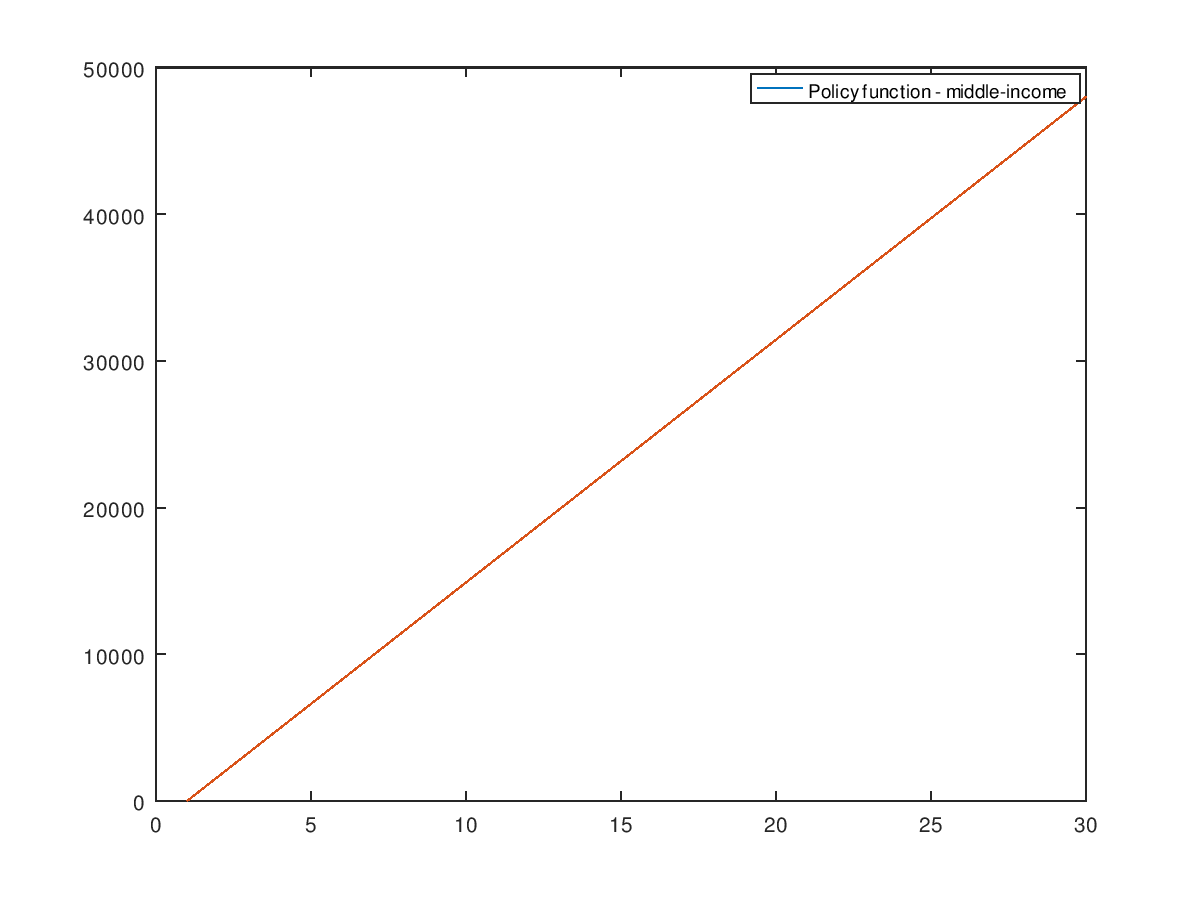
\includegraphics[scale=0.5]{figure1.png}

  \subsection{Part B}

  The super-rich are much less likely to run into the borrowing constraint when calculating desired consumption, so they should have essentially linear savings behavior. Blue-collar workers are more likely to run into the borrowing constraint, and so have non-linear savings behavior with little assets due to precautionary motives.

  Figures are missing because code does not appear to converge.

  \includegraphics[scale=0.25]{figure2.png}
  \includegraphics[scale=0.25]{figure3.png}

  \subsection{Part E}

  Blue-collar workers are now less likely to run into the borrowing constraint when calculating desired consumption, and so are willing to save less at every point on the asset grid because the precautionary motive is not as strong.

  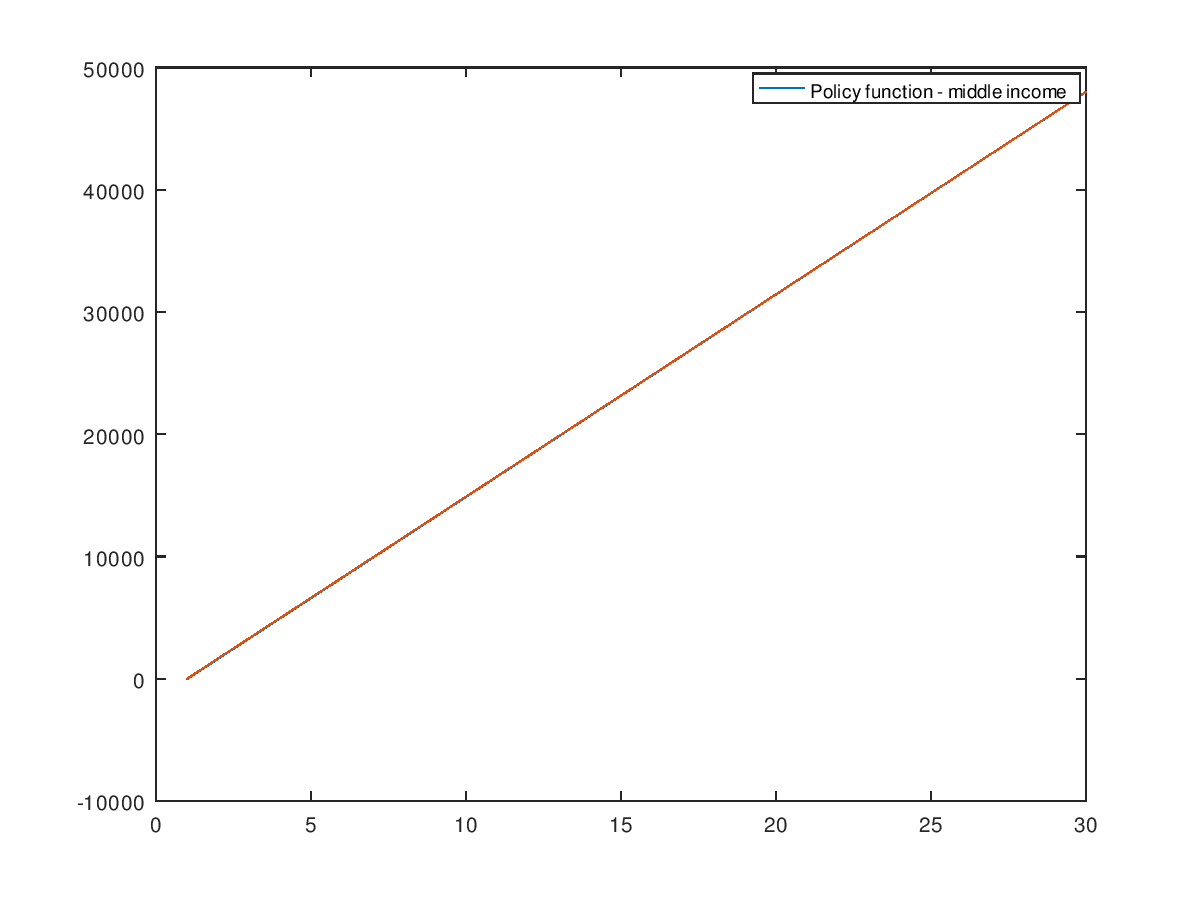
\includegraphics[scale=0.5]{figure4.png}

  \subsection{Part F}

  Workers are now much more risk-averse, so they save more in response to precautionary motives at every point on the asset grid. The superrich still display essentially linear savings behavior.

  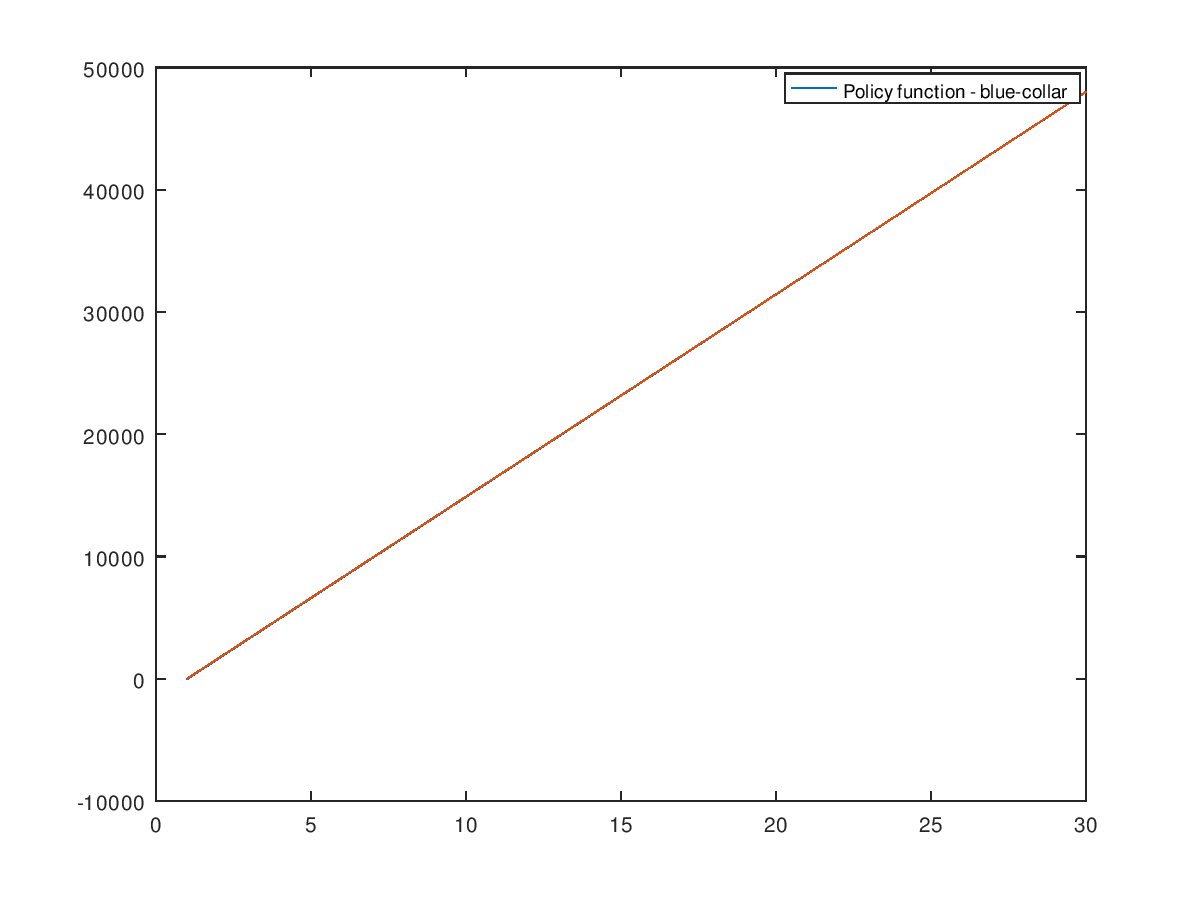
\includegraphics[scale=0.5]{figure5.png}

  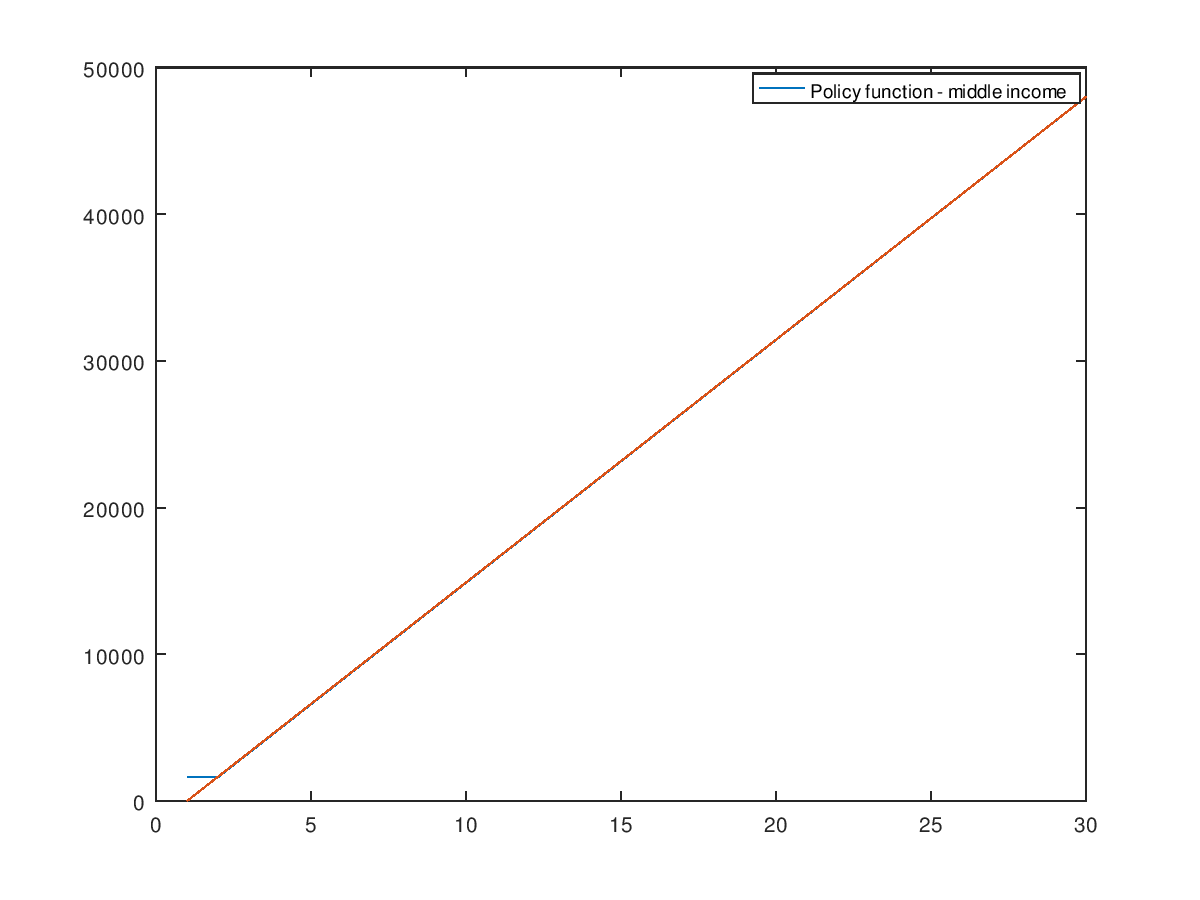
\includegraphics[scale=0.25]{figure6.png}
  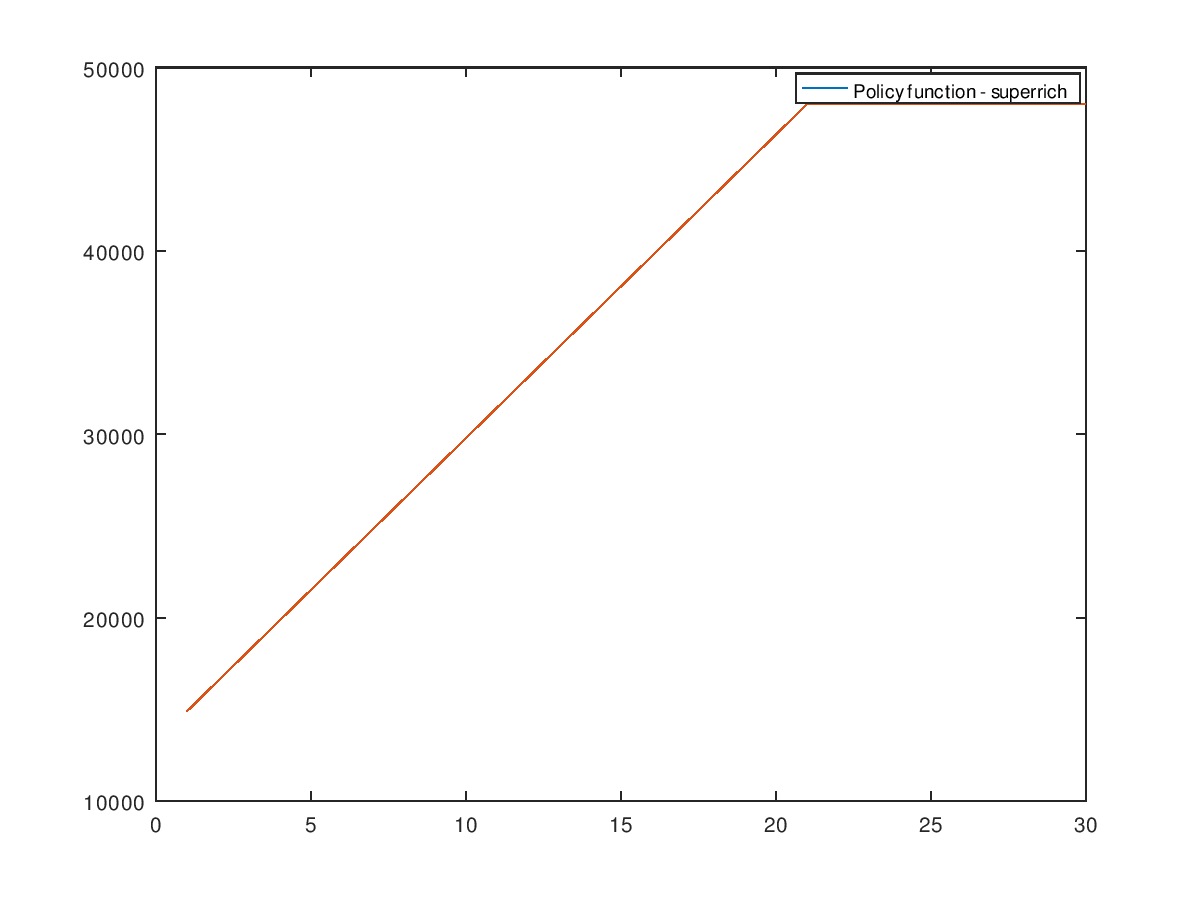
\includegraphics[scale=0.25]{figure7.png}


  \appendix

Matlab Code

\begin{lstlisting}[breaklines]
clear all
clc

sigma=2;
sigma1=10;
rho=0.975;
beta=0.93;
R=1.025;
y1=16000;
y2=80;
y3=15;
y = [y1, y2, y3];
Gamma = [ 0.02, 0.98, 0; 0.001, 0.78, 0.219; 0, 0.036, 0.964 ];
abar = 0;
abar2 = -30;
ymax = 3*y1;
m1 = 30;
m2 = 500;

a= linspace(abar, ymax, m1);
aa = linspace(abar, ymax, m2);
aaa = linspace(abar2, ymax, m1);
aaaa = linspace(abar2, ymax, m1);

A0 = a(m1)*ones(m1,length(y));
A1 = aa(m2)*ones(m2,length(y));
A2 = aaa(m1)*ones(m1,length(y));
A3 = aaaa(m1)*ones(m1,length(y));

%Initial guesses
a0=zeros(length(a),3);
a1=zeros(length(aa),3);
a2=zeros(length(aaa),3);
a3 = zeros(length(aaaa),3);

for i=1:length(a);
a0(i,:)=a(i);
a2(i,:)=a(i);
a3(i,:) = a(i);
end
for i=1:length(a2);
  a1(i,:) = a(i);
end

Diff = 100;
tol = 1e-3;
%
%



tic
while Diff > tol

    for i = 1:length(y)
        for h = 1:length(a)
            c1 = R*a(h) + y(i) - a(1);
            c2 = R*a(1) + y - a0(1,:);
            E1 = c1.^(-sigma) - rho*beta*R*sum( Gamma(i,:).*c2.^(-sigma) );

            if E1>0
                A0(h,i) = a(1);
            else

                delta = -100;
                DELTA = NaN(length(a),1);
                k = 0;

                while delta<0 & k<length(a)
                    k = k+1;
                    c1 = R*a(h) + y(i) - a(k);
                    c2 = R*a(k) + y - a0(k,:);
                    delta = max(0,c1).^(-sigma) - rho*beta*R*sum( Gamma(i,:).*max(0,c2).^(-sigma));
                    DELTA(k)=delta;
                end

                if abs( DELTA(k) )>abs( DELTA(k-1) )
                    A0(h,i) = a(k-1);
                else
                    A0(h,i) = a(k);
                end

            end
        end
    end

    Diff = max(max(abs(A0-a0)));
    a0 = A0;

end
toc

Diff = 100;
tol = 1e-3;

aprime=A0;
line=a;
figure(1)
plot(aprime(:,2));
legend('Policy function - middle-income');
hold on
plot(line)
hold off
saveas(figure(1),'figure1.jpg')


tic
while Diff > tol

    for i = 1:length(y)
        for h = 1:length(aa)
            c3 = R*aa(h) + y(i) - aa(1);
            c4 = R*aa(1) + y - a1(1,:);
            E1 = c3.^(-sigma) - rho*beta*R*sum( Gamma(i,:).*c4.^(-sigma) );

            if E1>0
                A1(h,i) = aa(1);
            else

                delta = -100;
                DELTA = NaN(length(aa),1);
                k = 0;

                while delta<0 & k<length(aa)
                    k = k+1;
                    c3 = R*aa(h) + y(i) - aa(k);
                    c4 = R*aa(k) + y - a1(k,:);
                    delta = max(0,c3).^(-sigma) - rho*beta*R*sum( Gamma(i,:).*max(0,c4).^(-sigma));
                    DELTA(k)=delta;
                end
                if k<2
                  A1(h,i) = aa(k)
                elseif abs( DELTA(k) )>abs( DELTA(k-1) )
                    A1(h,i) = aa(k-1);
                else
                    A1(h,i) = aa(k);
                end

            end
        end
    end

    Diff = max(max(abs(A1-a1)));
    a1 = A1;

end
toc



Diff = 100;
tol = 1e-3;


aprime1=A1;
line=aa;
figure(2)
plot(aprime1(:,3));
legend('Policy function - superrich');
hold on
plot(line)
hold off
saveas(figure(2),'figure2.jpg')

figure(3)
plot(aprime1(:,1));
legend('Policy function - blue-collar);')
hold on
plot(line)
hold off
saveas(figure(3),'figure3.jpg')

tic
while Diff > tol

    for i = 1:length(y)
        for h = 1:length(aaa)
            c5 = R*aaa(h) + y(i) - aaa(1);
            c6 = R*aaa(1) + y - a2(1,:);
            E1 = c5.^(-sigma) - rho*beta*R*sum( Gamma(i,:).*c6.^(-sigma) );

            if E1>0
                A2(h,i) = aaa(1);
            else

                delta = -100;
                DELTA = NaN(length(aaa),1);
                k = 0;

                while delta<0 & k<length(aaa)
                    k = k+1;
                    c5 = R*aaa(h) + y(i) - aaa(k);
                    c6 = R*aaa(k) + y - a2(k,:);
                    delta = max(0,c5).^(-sigma) - rho*beta*R*sum( Gamma(i,:).*max(0,c6).^(-sigma));
                    DELTA(k)=delta;
                end
                if k<2
                  A2(h,i) = aaa(k);
                elseif abs( DELTA(k) )>abs( DELTA(k-1) )
                    A2(h,i) = aaa(k-1);
                else
                    A2(h,i) = aaa(k);
                end

            end
        end
    end

    Diff = max(max(abs(A2-a2)));
    a2 = A2;

end
toc

Diff = 100;
tol = 1e-3;


aprime2=A2;
line=aaa;
figure(4)
plot(aprime2(:,3));
legend('Policy function - middle income');
hold on
plot(aprime(:,3));
hold off
saveas(figure(4),'figure4.jpg')

tic
while Diff > tol

    for i = 1:length(y)
        for h = 1:length(aaaa)
            c7 = R*aaaa(h) + y(i) - aaaa(1);
            c8 = R*aaaa(1) + y - a3(1,:);
            E1 = c7.^(-sigma1) - rho*beta*R*sum( Gamma(i,:).*c8.^(-sigma1) );

            if E1>0
                A3(h,i) = aaaa(1);
            else

                delta = -100;
                DELTA = NaN(length(aaa),1);
                k = 0;

                while delta<0 & k<length(aaa)
                    k = k+1;
                    c7 = R*aaaa(h) + y(i) - aaaa(k);
                    c8 = R*aaaa(k) + y - a3(k,:);
                    delta = max(0,c7).^(-sigma1) - rho*beta*R*sum( Gamma(i,:).*max(0,c8).^(-sigma1));
                    DELTA(k)=delta;
                end
                if k<2
                  A3(h,i) = aaaa(k);
                elseif abs( DELTA(k) )>abs( DELTA(k-1) )
                    A3(h,i) = aaaa(k-1);
                else
                    A3(h,i) = aaaa(k);
                end

            end
        end
    end

    Diff = max(max(abs(A3-a3)));
    a3 = A3;

end
toc

aprime3=A3;
line=aaaa;
figure(5)
plot(aprime3(:,3));
legend('Policy function - blue-collar');
hold on
plot(aprime(:,3));
hold off
saveas(figure(5),'figure5.jpg')

figure(6)
plot(aprime3(:,2));
legend('Policy function - middle income');
hold on
plot(aprime(:,2));
hold off
saveas(figure(6),'figure6.jpg')

figure(7)
plot(aprime(:,1));
legend('Policy function - superrich');
hold on
plot(aprime(:,1));
hold off
saveas(figure(7),'figure7.jpg')
\end{lstlisting}


\end{document}
